%%%%%%%%%%%%%%%%%%%%%%%%%%%%%%%%%%%%%%%%%
% Programming/Coding Assignment
% LaTeX Template
%
% This template has been downloaded from:
% http://www.latextemplates.com
%
% Original author:
% Ted Pavlic (http://www.tedpavlic.com)
%
% Note:
% The \lipsum[#] commands throughout this template generate dummy text
% to fill the template out. These commands should all be removed when 
% writing assignment content.
%
% This template uses a Perl script as an example snippet of code, most other
% languages are also usable. Configure them in the "CODE INCLUSION 
% CONFIGURATION" section.
%
%%%%%%%%%%%%%%%%%%%%%%%%%%%%%%%%%%%%%%%%%

%----------------------------------------------------------------------------------------
%	PACKAGES AND OTHER DOCUMENT CONFIGURATIONS
%----------------------------------------------------------------------------------------

\documentclass{article}

\usepackage{fancyhdr} % Required for custom headers
\usepackage{lastpage} % Required to determine the last page for the footer
\usepackage{extramarks} % Required for headers and footers
\usepackage[usenames,dvipsnames]{color} % Required for custom colors
\usepackage{graphicx} % Required to insert images
\usepackage{listings} % Required for insertion of code
\usepackage{courier} % Required for the courier font
\usepackage{lipsum} % Used for inserting dummy 'Lorem ipsum' text into the template
\usepackage[utf8]{inputenc} % Required for inputting international characters
\usepackage[T1]{fontenc} % Output font encoding for international characters
\usepackage{pdfpages}

% Margins
\topmargin=-0.45in
\evensidemargin=0in
\oddsidemargin=0in
\textwidth=6.5in
\textheight=9.0in
\headsep=0.25in

\linespread{1.1} % Line spacing

% Set up the header and footer
\pagestyle{fancy}
\lhead{\hmwkTitle} % Top left header
\rhead{\hmwkAuthorName} % Top right header
%\chead{\hmwkClass\ (\hmwkClassInstructor\ \hmwkClassTime): \hmwkTitle} % Top center head
%\rhead{\firstxmark} % Top right header
\lfoot{\lastxmark} % Bottom left footer
\cfoot{} % Bottom center footer
\rfoot{Strana\ \thepage\ - \protect\pageref{LastPage}} % Bottom right footer
\renewcommand\headrulewidth{0.4pt} % Size of the header rule
\renewcommand\footrulewidth{0.4pt} % Size of the footer rule

\setlength\parindent{0pt} % Removes all indentation from paragraphs

%----------------------------------------------------------------------------------------
%	CODE INCLUSION CONFIGURATION
%----------------------------------------------------------------------------------------

\definecolor{MyDarkGreen}{rgb}{0.0,0.4,0.0} % This is the color used for comments
\lstloadlanguages{C++} % Load C++ syntax for listings
\lstset{language=C++, % Use c++ in this example
        frame=single, % Single frame around code
        basicstyle=\small\ttfamily, % Use small true type font
        keywordstyle=[1]\color{Blue}\bf, % c++ functions bold and blue
        keywordstyle=[2]\color{Purple}, % c++ function arguments purple
        keywordstyle=[3]\color{Blue}\underbar, % Custom functions underlined and blue
        identifierstyle=, % Nothing special about identifiers                                         
        commentstyle=\usefont{T1}{pcr}{m}{sl}\color{MyDarkGreen}\small, % Comments small dark green courier font
        stringstyle=\color{Purple}, % Strings are purple
        showstringspaces=false, % Don't put marks in string spaces
        tabsize=5, % 5 spaces per tab
        %
        % Put standard c++ functions not included in the default language here
        morekeywords={rand},
        %
        % Put c++ function parameters here
        morekeywords=[2]{on, off, interp},
        %
        % Put user defined functions here
        morekeywords=[3]{test},
       	%
        morecomment=[l][\color{Blue}]{...}, % Line continuation (...) like blue comment
        numbers=left, % Line numbers on left
        firstnumber=1, % Line numbers start with line 1
        numberstyle=\tiny\color{Blue}, % Line numbers are blue and small
        stepnumber=5 % Line numbers go in steps of 5
}

% Creates a new command to include a perl script, the first parameter is the filename of the script (without .pl), the second parameter is the caption
\newcommand{\perlscript}[2]{
\begin{itemize}
\item[]\lstinputlisting[caption=#2,label=#1]{#1.pl}
\end{itemize}
}

%----------------------------------------------------------------------------------------
%	DOCUMENT STRUCTURE COMMANDS
%	Skip this unless you know what you're doing
%----------------------------------------------------------------------------------------

% Header and footer for when a page split occurs within a problem environment
\newcommand{\enterProblemHeader}[1]{
\nobreak\extramarks{#1}{#1 pokračování na další straně\ldots}\nobreak
\nobreak\extramarks{#1 (pokračování)}{#1 pokračování na další straně\ldots}\nobreak
}

% Header and footer for when a page split occurs between problem environments
\newcommand{\exitProblemHeader}[1]{
\nobreak\extramarks{#1 (pokračování)}{#1 pokračování na další straně\ldots}\nobreak
\nobreak\extramarks{#1}{}\nobreak
}

%----------------------------------------------------------------------------------------
%	NAME AND CLASS SECTION
%----------------------------------------------------------------------------------------

\newcommand{\hmwkTitle}{Geometrické vyhledávání bodu} % Assignment title
\newcommand{\hmwkDueDate}{Datum odevzdání: 13.11.2017} % Due date
\newcommand{\hmwkClass}{155ADKG} % Course/class
%\newcommand{\hmwkClassTime}{10:30am} % Class/lecture time
%\newcommand{\hmwkClassInstructor}{Jones} % Teacher/lecturer
\newcommand{\hmwkAuthorName}{Petra~Millarová, Bc.~Oleksiy~Maybrodskyy} % Your name

%----------------------------------------------------------------------------------------
%	TITLE PAGE
%----------------------------------------------------------------------------------------

\title{
\vspace{2in}
\textmd{\textbf{\hmwkClass:\ \hmwkTitle}}\\
\normalsize\vspace{0.1in}\large{\hmwkDueDate}\\
%\vspace{0.1in}\large{\textit{\hmwkClassInstructor\ \hmwkClassTime}}
\vspace{3in}
}

\author{\textbf{\hmwkAuthorName}}
\date{} % Insert date here if you want it to appear below your name

%----------------------------------------------------------------------------------------

\begin{document}

\maketitle

%----------------------------------------------------------------------------------------
%	TABLE OF CONTENTS
%----------------------------------------------------------------------------------------

%\setcounter{tocdepth}{1} % Uncomment this line if you don't want subsections listed in the ToC

\newpage
\tableofcontents
\newpage

%----------------------------------------------------------------------------------------
%	PROBLEM 1
%----------------------------------------------------------------------------------------

% To have just one problem per page, simply put a \clearpage after each problem

\section{Zadání}
\indent Následuje kopie oficiálního zadání úlohy. Autoři z nepovinných bodů zadání implementovali všechny kromě algoritmu pro automatcké generování nekonvexních polygonů.
\begin{figure}[htbp]
    \centering
        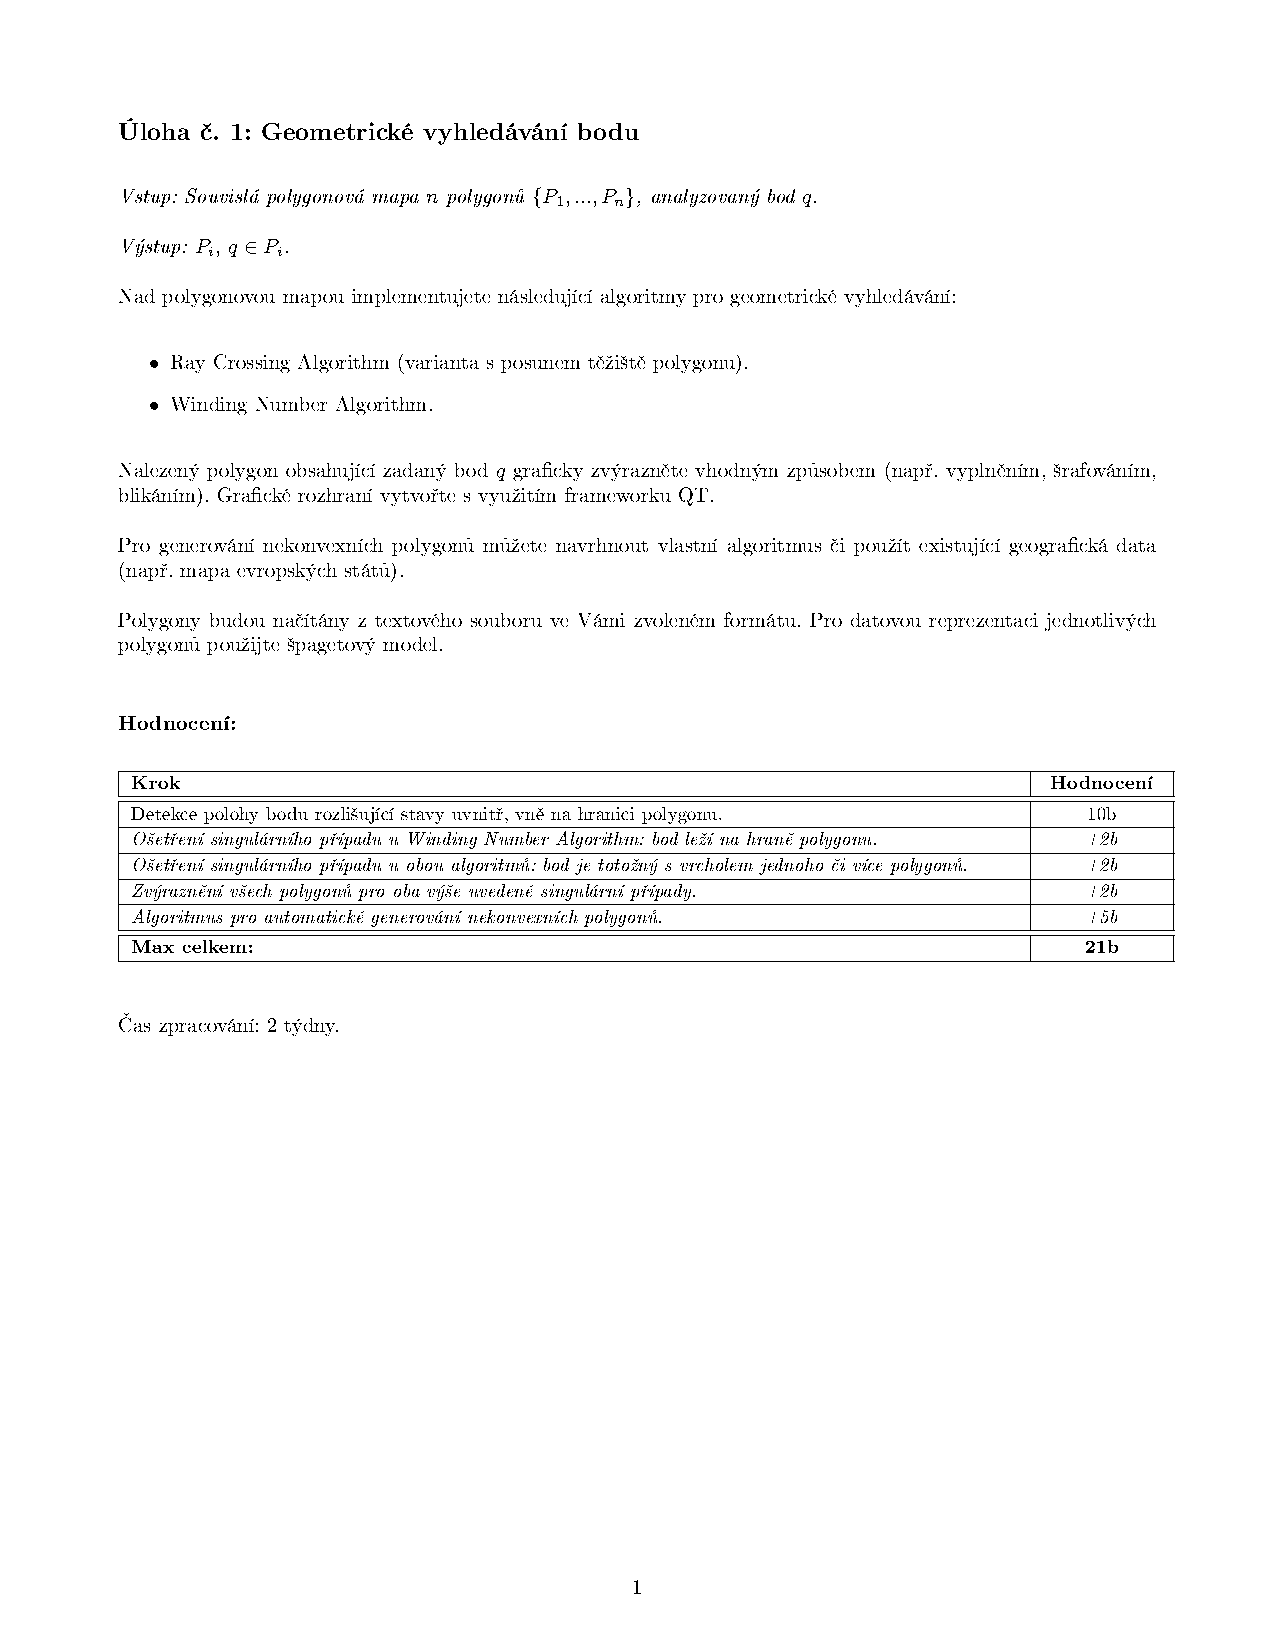
\includegraphics[clip, trim=0cm 11cm 0cm 0cm, width=1.00\textwidth]{zadani.pdf}
\end{figure}
\clearpage
\section{Popis a rozbor problému} %+vzorce
\indent 
Tato úloha se věnuje řešení praktického problému určování pozice uživatelem zadaného bodu $q$ vůči polygonům načteným ze souboru. Jako implementaci si lze zjednodušeně představit zjišťování polohy konkrétního bodu kliknutím na digitální mapě. 
\\
\\
\textsl{Nechť existuje pole ve dvojrozměrné kartézské soustavě s \textbf n body. Uzavřením tohoto pole vznikne polygon. Polygon může nabývat jak konvexní, tak nekonvexní tvar.}
\\
\\
Polygon je konvexní právě tehdy, když poloha všech bodů je vůči jakékoliv přímce procházející vedle polygonu, vždy na stejné straně. 

Rozdíl mezi \textsl konvexním a  \textsl nekonvexním polygonem je možné názorně vidět na obrázcích níže.
\begin{figure}[htbp]
\centering
        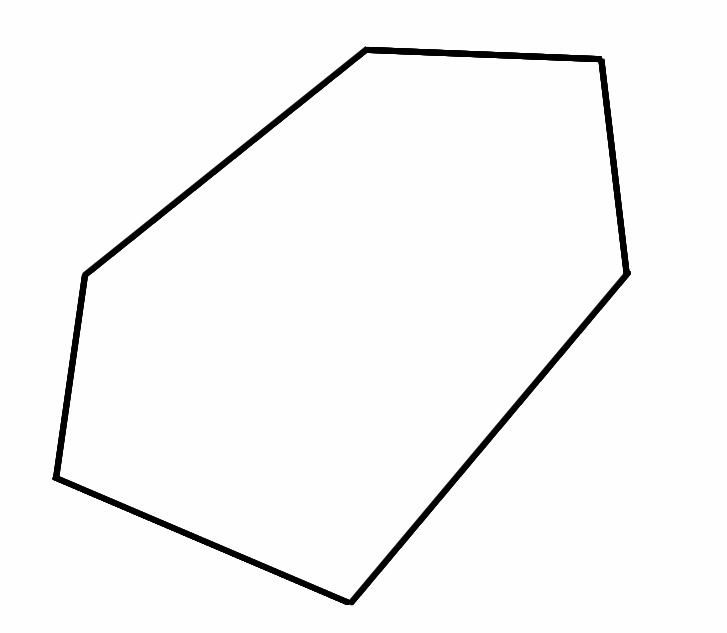
\includegraphics[clip, trim=0cm 0cm 0cm 0cm, width=0.2500\textwidth]{obrazek1.png}
 
\includegraphics[clip, trim=0cm 0cm 0cm 0cm, width=0.2500\textwidth]{obrazek2.png}
\end{figure}
\bigskip
\begin{center}
obr 1.:\textsl{konvexní polygon (vlevo) a nekonvexní polygon (vpravo)}
\end{center}
Pokud následně polygon rozdělíme na menší polygonové útvary, pak polohu zvoleného bodu $q$ můžeme popsat následovně: 
\begin{enumerate}
\item   Bod $q$ se nachází uvnitř polygonu  $q {\in} P_i$ 
\item   Bod $q$ se nachází vně všech polygonů  $q {\not \in} P_i$ 
\item   Bod se nachází na hraně jednoho  $q {\not \in} P_i$ nebo dvou polygonů $q {\in} P_{i,i+1}$ 
\item   Bod je totožný s vrcholem jednoho polygonu nebo více polygonů $q {\in} P_{i,i+1,...,i+n}$
\end{enumerate}
Výpočet se bude provádět na základě metod \textbf {Ray Crossing algorithm} a  \textbf {Winding Number algorithm}. Jejich výpočet je popsán v následujících kapitolách. 
\\
\clearpage
\section{Popisy algoritmů} %formálním jazykem
V dané úloze jsou použity následující algoritmy, avšak existují i další možnosti, jak polohu bodu určit (metoda pásů, Line Sweep algorithm aj.)
\subsection{Ray crossing algorithm}
\textsl{Nechť existuje uzavřený polygon ve dvojrozměrné kartézské soustavě, tvořený \textbf n body. Nechť následně existuje bod q, kteréhož polohu se snažime určit. Proložíme-li bodem q nekonečný počet paprsků směrem k polygonu, pak pro jednotlivý paprsek nastane jedna z následujících situací: }
\begin{enumerate}
\item   počet průsečíků paprsku  $k$ je roven sudému počtu, pak se bod $q$ nachází vně polygonu  $q {\not \in} P_i$ 
\item  počet průsečíků paprsku  $k$ je roven lichému počtu, pak se bod $q$ nachází uvnitř polygonu  $q \in P_i$
\end{enumerate} 
Zároveň mohou nastat singularity, respektive jisté situace, kdy algoritmus "nefunguje" a nedokáže přímo nalézt správný výsledek. V algoritmu ray crossing se konkrétně jedná o tyto případy:
\begin{enumerate}
\item   Bod se nachází na hraně jednoho  $q {\in} P_i$ nebo dvou polygonů $q {\in} P_{i,i+1}$ 
\item   Bod je totožný s vrcholem jednoho polygonu nebo více polygonů $q {\in} P_{i,i+1,...,i+n}$
\end{enumerate} 
Řešením je posun, respektive redukce vrcholů polygonů směrem k poloze bodu  $q$.
\\
Hledáný algoritmus je možné popsat následovně:
\begin{enumerate} 

\item Inicializace bodů polygonu $p_i$, počet průsečíku = 0;

\item Redukce souřadnic $x$ bodů polygonu k bodu $q$,  respektivě k paprskovému segmentu, $x_i^{'} = x_i - x_q$. 

\item  Redukce souřadnic $y$ bodů polygonu k bodu $q$, respektivě k paprskovému segmentu, $y_i^{'} = y_i - y_q$. 

\item Znovu pro ostatní body daného polygonu $p_i$/ 

\item if $(y_{i}^{'} <= 0)\&\&(y_i+1^{'} > 0)\|(y_{i}^{'} > 0)\&\&(y_i+1^{'} <= 0)$. 

\item $x_m^{'} = (x_i+1^{'}y_{i}^{'}-x_{i}^{'}y_i+1^{'})/(y_{i+1}^{'}-y_{i}^{'})$. 

\item Sčítaní počtu redukováných bodů, pro $x_i^{'} > 0$  


\item Pokud je počet průsečíku sudý, pak $q \in P$, pokud není, pak  $q \notin P$ 

\end{enumerate} 
\clearpage
\newpage 

\subsection{Winding Number Algorithm} 
\textsl{Nechť existuje uzavřený polygon ve dvojrozměrné kartézské soustavě, tvořený pomocí \textbf n bodů. Nechť následně existuje bod q, polohu kteréhož se snažíme určit. Z pohledu bodu $q$ provedeme orientaci směru, ze které se pak následně určí součet všech úhlů na jednotlivé body uvedeného polygonu.}
\\
\\
Součtový úhel bude dále značen jako $w$. Výpočet je lepší provádět proti směru hodinových ručiček, jelikož v případě tohoto směru hodnota počítaných oběhů Winding Number $\Omega$  nabývá kladných hodnot. Je třeba také pamatovat, že hodnota $\Omega$ je uváděna v počtech oběhů a je záporná při oběhu po směru 
hodinových ručiček a kladná ve směru opačném. Do výpočtu také vstupuje tolerance $\epsilon$, která zahrnuje chyby vzniklé zaokrouhlováním a strojovou přesností. Dle uvedených matematických podmínek mohou nastat následující případy:
\begin{enumerate} 
\item $w$=\textbf {2R}, pak $q \in P_i$ 
\item  $w$ < \textbf {2R}, pak $q {\not \in} P_i$
\end{enumerate}
 Níže je uveden algoritmus výpočtu: 

\begin{enumerate} 

\item Vstup $\omega = 0$, tolerance $\epsilon$

\item Orientace z bodu $q$ káždého následujícího bodu  $p_{i+1}$ od orientaci na bod $p_i$

\item Určení úhlu $\omega_i = \angle p_i, q, p_{i+1}$ 

\item  $\omega = \omega + \omega_i$, pro bod vprávo od orientace na bod $p_i$, pokud je bod vlevo od orientace na bod $p_i$, pak $\omega = \omega - \omega_i$

\item Pokud platí podmínka $(\left|\omega - 2\Pi \right| < \epsilon)$, pak $q \in P$

\item Pokud neplatí podmínka  $(\left|\omega - 2\Pi \right| < \epsilon)$, pak $q \notin P$

\end{enumerate} 
\clearpage
\newpage
\section{Problematické situace a singularity} %rozbor a osetreni v kodu
\subsection{Bod ležící na hraně polygonu} 

\bigskip 

Pokud vyjdeme z podmínky, že bod se nachází na hraně polygonu, pak z pohledu geometrie je jasné, že svýrající úhel mezi krajnými body dané hrany bude roven $R$ neboli. Pokud ale ještě zavedeme chybu toleranci $\epsilon$, pak $R+\epsilon$. Jelikož bod leží na hraně, pak zároveň patří do obou polygonů.

\subsection{Bod je identický s vrcholem jednoho až n polygonů} 

\bigskip 

Byl proveden prohledávácí test, jestli souřadnice bodu  $q$ jsou identické se souřadnicemi kterého koliv polygonu. Pokud test byl úspěšný, pak se již dále neprováděl a rovnou se vybarvil konkretní polygon. Pokud během testu se ukazalo, že souřadnice jsou identické s vrcholem, který je společný pro několik polygonů, pak se vybarvilo hned několik polygonů.
\begin{figure}[htbp]
\centering
        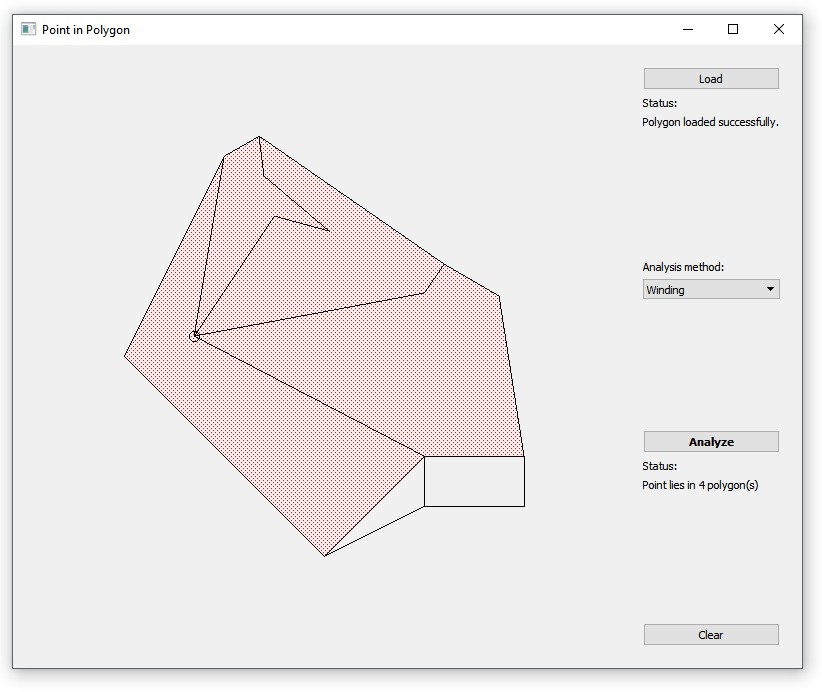
\includegraphics[clip, trim=0cm 0cm 0cm 0cm, width=1\textwidth]{more.jpg}
\end{figure}

\section{Vstupní data}
Do programu vstupují dvě odlišné hodnoty: 
\begin{enumerate} 
\item analyzovaný bod \textit{\textbf {q}}. 
\item soubor polygonů. 
\end{enumerate} 

Analyzovaný bod \textit{\textbf {q}}, vstupuje na základě ručního vstupu přes GUI, tedy zmačknutím levého tlačítka myší v grafickém okně.
\\
Vstupní (.txt) soubor obsahuje polygony zadané jednotlivými body.

\bigskip 

 \textit{\textbf {Složený vstupných dat .txt:}}
První řádek obsahuje počet vstpujících polygonů souřanici \textit{\textbf {X}}
\\
Druhý řádek obsahuje počet bodů prvního polygonu
\\
Třetý řádek obsahuje vypsané souřadnice  \textit{\textbf {X}} vstupního polygonu
\\
Čtvrtý řádek obsahuje vypsané souřadnice  \textit{\textbf {Y}} vstupního polygonu
\bigskip 
\\
Další řádek obsahuje počet bodů druhého polygonu, nasledující vstup je identický se vstupem prvního polygonu
\bigskip 

Při vstupu textového souboru program již rovnou rozezná počet vstupných polygonů a jejích rozměry, což značně ulehčuje následující prací. Vstupní souřadnice mohou být, jak celočíselné, tak s desetinou tečkou. Souřadnice \textit{\textbf {X}} a \textit{\textbf {Y}} se sekvenčně ukládají do 
proměnné \textbf {QPoint}, která se ukládá do proměnné vektoru typu  \textbf {std::vector<QPoint>}, který znázorňuje polygon, který  se následně ukláda do proměnné typu  \textbf {std::vector<vector<QPoint>}\textbf {>}, která sloučuje všechny polygony. 


\section{Výstupní data}
	Výstup je vizualizací řešeného problému v grafickém okně. Taky v grafickém okně je slovně popsano, do kolika polygonu náleží hledaný bod.\\ 
\bigskip 

Po načtení vstupních dat \textit{\textbf {Load}}, v pravém horním rohu grafického 
okna, se polygony ihned vykreslí a po libovolným kliknutí levého tlačítka myši se vykreslí také vstupní 
bod.\\ 
Podle výsledků daného testu se červeně zvýrazní polygony, do kterých patří hledaný bod.
\clearpage
\section{Ukázky aplikace} %printscreen
\begin{figure}[htbp]
\centering
        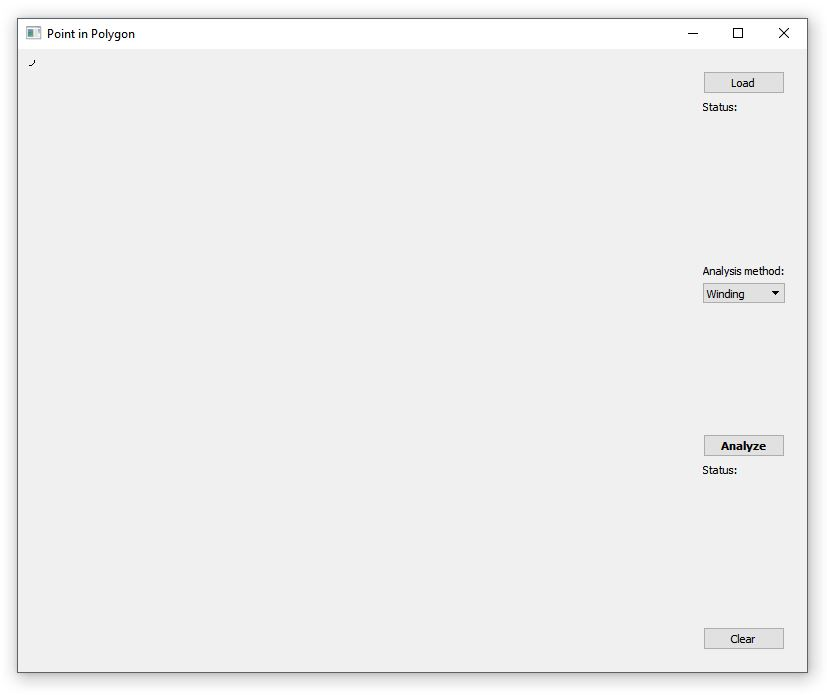
\includegraphics[clip, trim=0cm 0cm 0cm 0cm, width=1\textwidth]{empty_app.jpg}
        \caption{Aplikace po spuštění}
\end{figure}
\begin{figure}[htbp]
\centering
        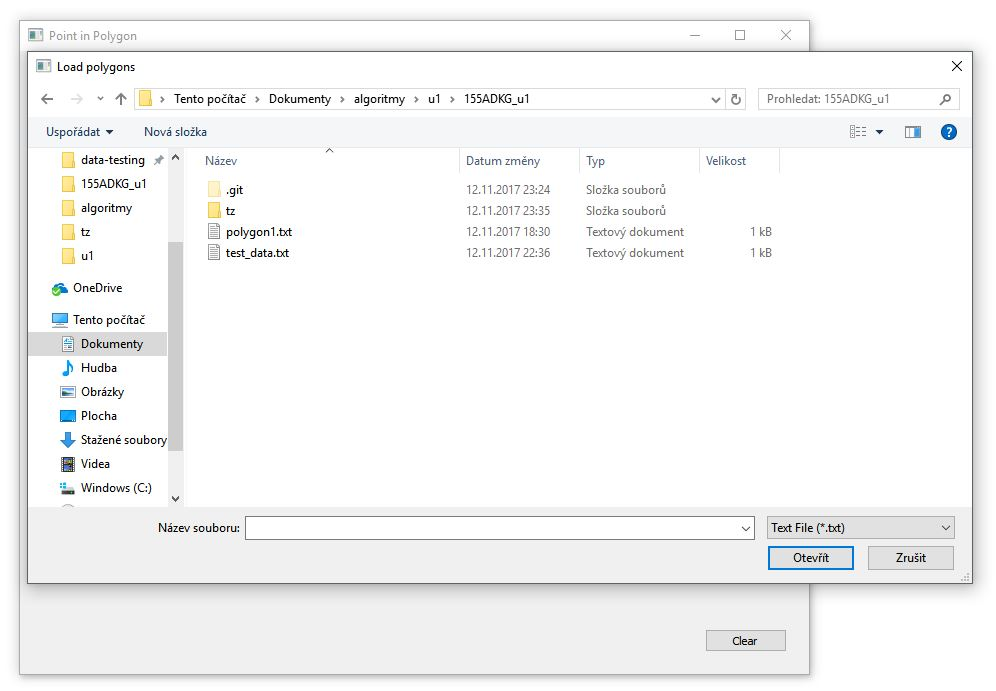
\includegraphics[clip, trim=0cm 0cm 0cm 0cm, width=1\textwidth]{load.jpg}
        \caption{Načtení dat}
\end{figure}
\begin{figure}[htbp]
\centering
        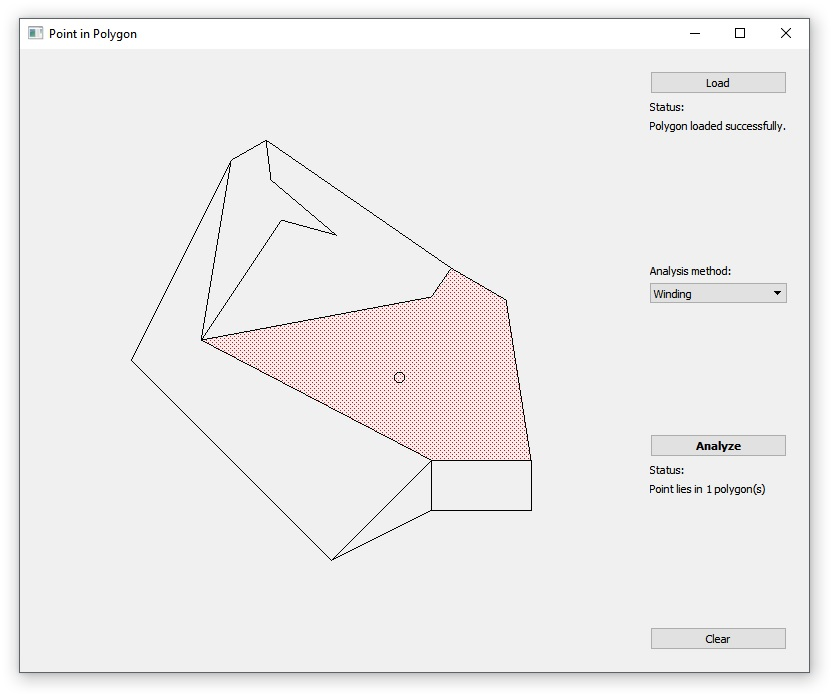
\includegraphics[clip, trim=0cm 0cm 0cm 0cm, width=1\textwidth]{analyzed.jpg}
        \caption{Po načtení a stisknutí tlačítka "Analyze"}
 \end{figure}       
        \begin{figure}[htbp]
\centering
        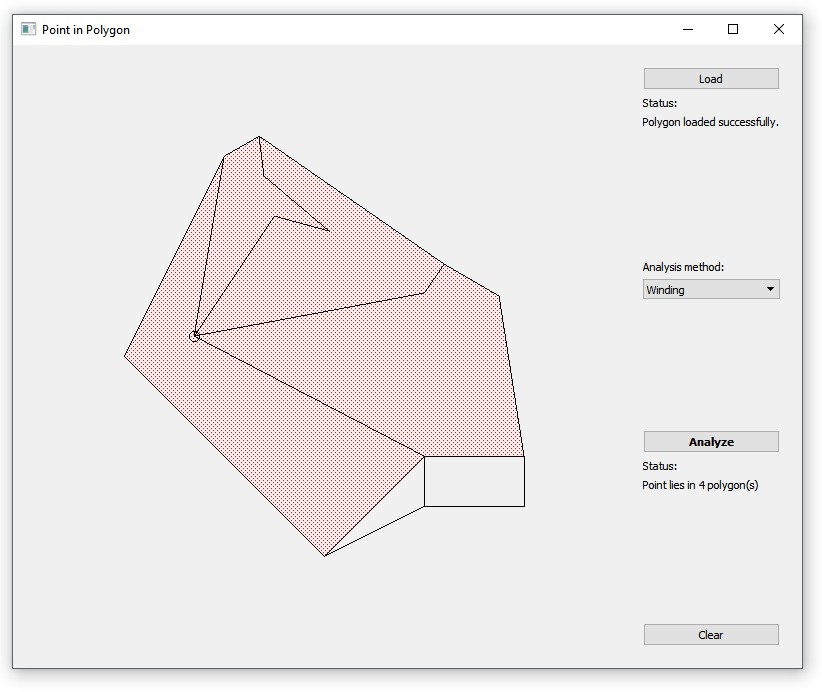
\includegraphics[clip, trim=0cm 0cm 0cm 0cm, width=1\textwidth]{more.jpg}
        \caption{"Výstup s více polygony"}
\end{figure}
\clearpage
\section{Závěr}
\indent Autoři splnili většinu bodů zadání a vznikl program, který načítá soubor polygonů, následně uživatele nechá umístit bod a po stisknutí tlačítka urči, zda a ve kterých polygonech bod leží. 
	\subsection{Náměty na vylepšení} %+možné či neřešené problémy
	\indent Aplikace, ač funkční a splňující daný účel, má spoustu nedostatků, které by bylo dobré v budoucnu odstranit. Autoři zde uvádí pár těch nejzjevnějších. \\
	\indent \textit{Vykreslování dat:} Aplikace bez problému vykreslí body, které se vejdou do jejího okna 665x605px. Problém nastává až tehdy, když jsou souřadnice větší než tato hodnota. Tato chyba jde odstranit vhodnou transformací okna (nebo souřadnic), která by ale probíhala na základě načtených dat. \\
	\indent \textit{Souřadnicové osy: } Vykreslovací okno má v Qt, stejně jako ve většině podobných nástrojů, počátek souřadnic v levém horním rohu, kladnou osu x vpravo a kladnou osu y směrem dolů. Tento model se však neshoduje ani s geodetickými souřadnicemi používanými na našem území (kladná y doleva, kladná x dolů), ani s klasickým označením os (kladná x doprava, kladná y nahoru). Proto se body v současné verzi zobrazují jinak, než by možná uživatel očekával. Vhodným řešením by byla opět transformace. \\
	\indent \textit{Přesnější souřadnice:} V současném stavu aplikace sice načítá data ve formátu \texttt{double}, avšak datová struktura \texttt{std::vector<std::vector<QPoint>>} body načítá bez desetinných míst jako typ \texttt{int}. V Qt knihovnách existuje i datový typ \texttt{QPointF}, který ukládá body jako typ \texttt{float}. Změně však bude potřeba přizpůsobit porovnávání čísel v algoritmech.
\bibliography{u1}
\bibliographystyle{plain}
\addcontentsline{toc}{section}{References}
\pagestyle{empty}

%\end{homeworkSection}
\clearpage

%-----------------------------------------------------------------------------
\end{document}